% Probably doesn't justify a separate section. Most people do not have it.

% Need more explanation with designs for both generalisation and atomisation.
% Including limitations.

\chapter{Implementation}

In this section, the architecture of the entire concept bottleneck pipeline, as well as more detail unrelated to logical modelling, is presented.
Since, the work in this thesis is a continuation of the previous unpublished work, laid out in \autoref{inherited-work}, this section may include some parts which do not constitute my work. 
The * sign is used to signify the work that is not the work of the author of the thesis.


\section{Concept Bottleneck Pipeline*}

% TODO: fix X in picture, add boxes for the three parts, missing outlining X as attention module
\begin{figure}[h]
\caption{The full pipeline for the classification of MLB-V2E dataset using concept bottleneck model (adapted from \cite{RefWorks:RefID:16-2021automatic})}
\centering
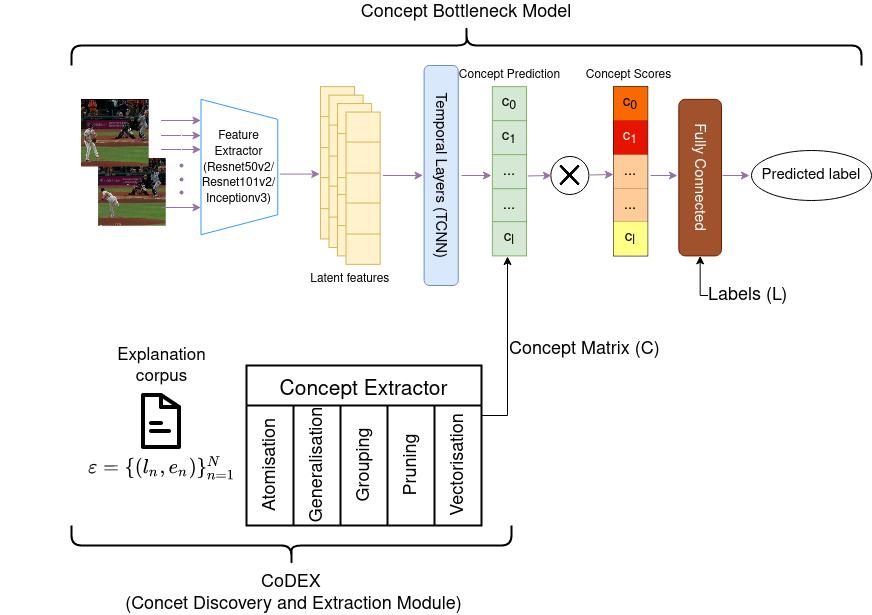
\includegraphics[width=\textwidth]{implementation/full architecture diagram.png}
\label{full-architecture-diagram}
\end{figure}

The concept bottleneck pipeline is shown in \ref{full-architecture-diagram}. 
Its purpose is to predict an output label correctly and in an interpretable manner.
The pipeline can be divided into concept extraction, concept prediction and label prediction pipeline. \\

\textbf{Concept Discovery and Extraction Pipeline (CoDEx)} is used to find an informative set of concepts for the problem at hand.
These concepts are extracted using human-generated explanations and labels in the dataset. 
The module consists of 5 parts: atomisation, generalisation, grouping, pruning, and vectorisation.

% INSERT chapter to reference.
The first two will be explained further in section X, while the latter 3 have been kept the same as explained in \autoref{inherited-work}. \\


\textbf{Concept Prediction Pipeline} has to predict the extracted concepts for the training images and varies depending on the problem type dealt with.
In all cases, it is a multi-label prediction model where output labels are probabilities that raw concepts occur.
The true labels for training are obtained from the concept matrix returned by the CoDEx module. \\

\textbf{Label Prediction Pipeline} has to predict the final output labels from the derived concepts. 
It consists of the attention mechanism, which highlights more relevant concepts for the prediction, and the fully connected layers. 
For further interpretability, the fully connected layer might be replaced with a neuro-symbolic component as a part of a future work.


\textbf{Atomistation/generalistion architecture}

% TODO: fix X in picture, add boxes for the three parts
\begin{figure}[h]
\caption{Simplified architecture for the concept generalisation part of the CoDEx pipeline.} 
\centering
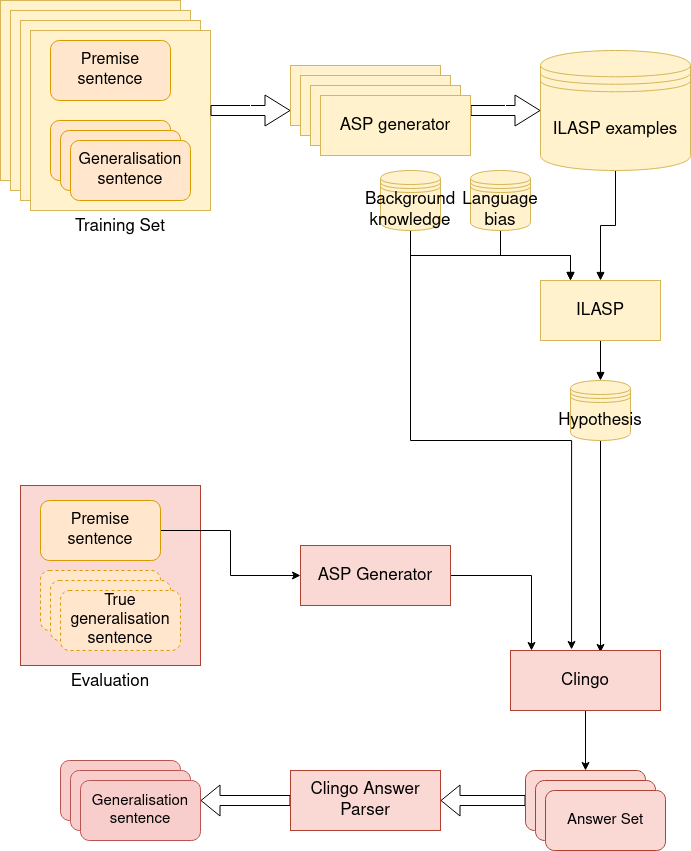
\includegraphics[width=\textwidth]{implementation/simplified architecture diagram.png}
\label{generalisation-architecture-diagram}
\end{figure}


The architecture diagram of the concept generalisation is shown in \ref{generalisation-architecture-diagram}.
% COLOUR into yellowish and redish
It can be divided into \textbf{learning} and \textbf{application/evaluation} stage.

The goal of the \textbf{learning} stage is to learn the hypothesis $H$ which will be able to generalise/atomise any sentence correctly.
Each training example for the learning stage consists of the premise and generalisation sentences provided in CSV format.
The raw examples are written in the following way:
\begin{center}
\setlength\parskip{0pt}
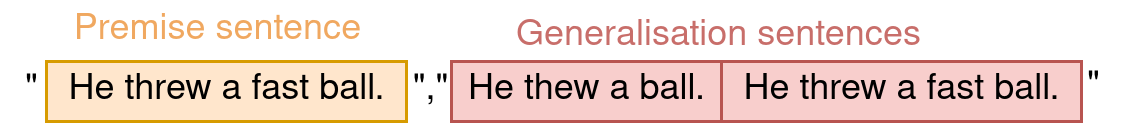
\includegraphics[width=.8\linewidth]{implementation/raw-generalisation-example.png}
\end{center}

% INSERT spacy/AlunNLP reference
The \textit{ASPGenerator} uses a NLP library to obtain the dependency graph of each sentence, used in the logical representation of an example.

The example files (\textit{ILASP examples} in \ref{generalisation-architecture-diagram}) are persisted since ILASP can only be run as a command line tool.
In addition, there ILASP examples can be split into multiple text files, commonly ten. 
% INSERT condor reference
The split of the files is used to run 10-fold cross validation experiments, which was parallelised using with Condor, a batch processing system.
% TODO: verify this - can be resolved immediately.
The final learned solution (hypothesis $H$), as is the standard practice when doing cross validation, has been produced by training the model using all of the examples.

% TODO: fix ASP Generator in image
The \textbf{application/evaluation} uses the learned hypothesis in order to split the unknown sentences.
In particular, the process consist of the following stages, visible in \ref{generalisation-architecture-diagram}:
 
 1. Conversion to the logical form. The sentences are converted to the logical form using in the equivalent manner as is the case for learning. In fact, the same module carries out both operations.
 
 % INSERT reference clingo
 2. Answer set solving. A sentence in the logical form, learned hypothesis and background knowledge are passed to Clingo answer set solver. Clingo will outputs all the answer sets of the provided program.
 
 3. Answer parsing. Each answer set returned corresponds to one generalisation/atomisation sentence. For each in\_generalised\_sent (or in\_atomised\_sent) token in an answer set, the actual word corresponding to that token is found. Words are joined in the same order as they appeared in the original sentence. Finally, post-processing techniques are applied to the resulting string, described in the next subsection, in order to fix possible grammatical issues. 
 
 
\subsubsection{Post-processing techniques}

% INSERT reference truecasing
Two post-processing techniques are used in order to return a grammatically correct sentence: punctuation addition and truecasing.

The \textbf{punct} tags are not provided for learning since the task becomes easier without them. 
As such, the punctuation addition simply adds the punctuation at the end of the learned sentence.
The punctuation added to each atomised/generalised sentence is the same as the punctuation of the original sentence.

% TODO: either reference stack overflow or find how I knew what I needed to capitalise.
Truecasing determines the true capitalisation where such information is unavailable.
% https://www.scribbr.com/language-rules/capitalization-rules/
As outlined in X, capitalisation is required for all proper nouns and for first words of sentences. 
The latter is simple to implement, while the former heavily relies on a part-of-speech tagger. 
% INSERT reference Penn Treebank
The implementation uses a POS tagger that assigns Penn Treebank tags to words which capture whether a noun is proper using \textit{NNP} (proper noun, singular) and \textit{NNPS} (proper noun, plural) tags.


% Briefly mention dependencies
% INSERT tags for all dependencies
\section{Dependencies}

% Modify this paragraph to talk about why we chose Answer Set Programming as a paradigm.



Majority of the code is written in Python due to the maturity libraries available for that language. 

The project depends on the following Python libraries to solve the needed problem. 
All Python dependencies are used through an adapter should they need to be replaced with an alternative in the future.
The dependencies needed were:

\textbf{SpaCy}: One of the most famous NLP libraries at the time of writing. 
It is used to determine part-of-speech tags of the tokens, create a dependency parse tree for a sentence and to split sentences. 
Abundance of documentation and ease of use were the determining factors for the selection of this library. 
An alternative such as AllenNLP could have been used if we needed more control over the actual models used.

\textbf{Sentence Transformers}: A library which provides access to pre-trained transformers. 
Since it is only used in the grouping stage, the ease of use of the library was the main reason for the selection of the library.

\textbf{PyFakeFS}: A library which mocks the file system. Used for testing some parts of the code.

Finally, \textbf{numpy}, \textbf{scikit-learn}, \textbf{matplotlib}, \textbf{panadas} which all are famous Python libraries used with AI projects. \\


% TODO: we need to talk about why we chose answer set programming  instead of some other paradigms / ILASP
Moreover, the code depends on the ILASP to learn an answer set program which generates the correct solution.
To be able to use the learned solution, we need an Answer set solver.
\textbf{Clingo} is the only Answer set solver in active development with a user guide so it was chosen.

